\chapter{Implementering}

\section{Hardware}
I dette kapitel beskrives kort, hvordan SRM'ens hardware og software komponenter er implementeret. Implementeringen afspejler designet, der er udarbejder under designfasen, se \nameref{bilag5}.  Til implementering af hardware komponenterne, er der valgt at illustrere en testopstilling ved hjælp af et diagram, inden kredsløbet bliver bygget på et fumlebræt. Denne testopstilling kan ses på figur \ref{fig:integrationstestDiagram}

\begin{figure}[H] 
\centering
{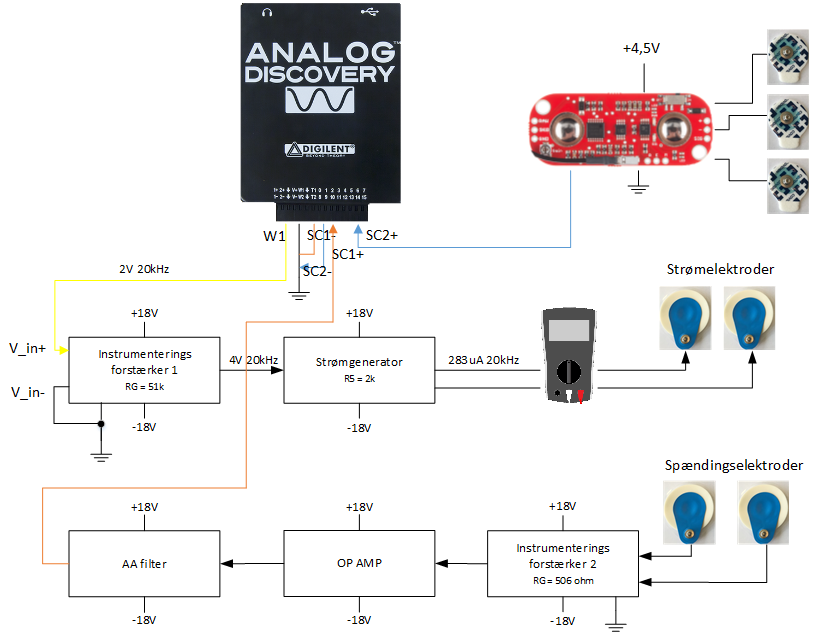
\includegraphics[width=\linewidth]
{Figure/integrationstestDiagram}}
\caption{Et diagram der illustrerer, hvordan hele systemets hardware komponenter skal implementeres på et fumlebræt. }
\label{fig:integrationstestDiagram}
\end{figure}

\pagebreak
Den overstående testopstilling blev efterfølgende bygget på fumlebrættet. På figur \ref{fig:integrationstestBilleder1} ses det fumlebrættet, et multimeter,  BI kredsløbet, EMG-måleren, forsyningsspændingen til kredsløbet, elektrode ledninger til hhv. BI kredsløbet og EMG-måleren. Fumlebrættet er tilkoblet til Analog Discovery'en, som bruges til både at forsyne BI kredsløbet og til dataopsamling. 


\begin{figure}[H]
\centering
{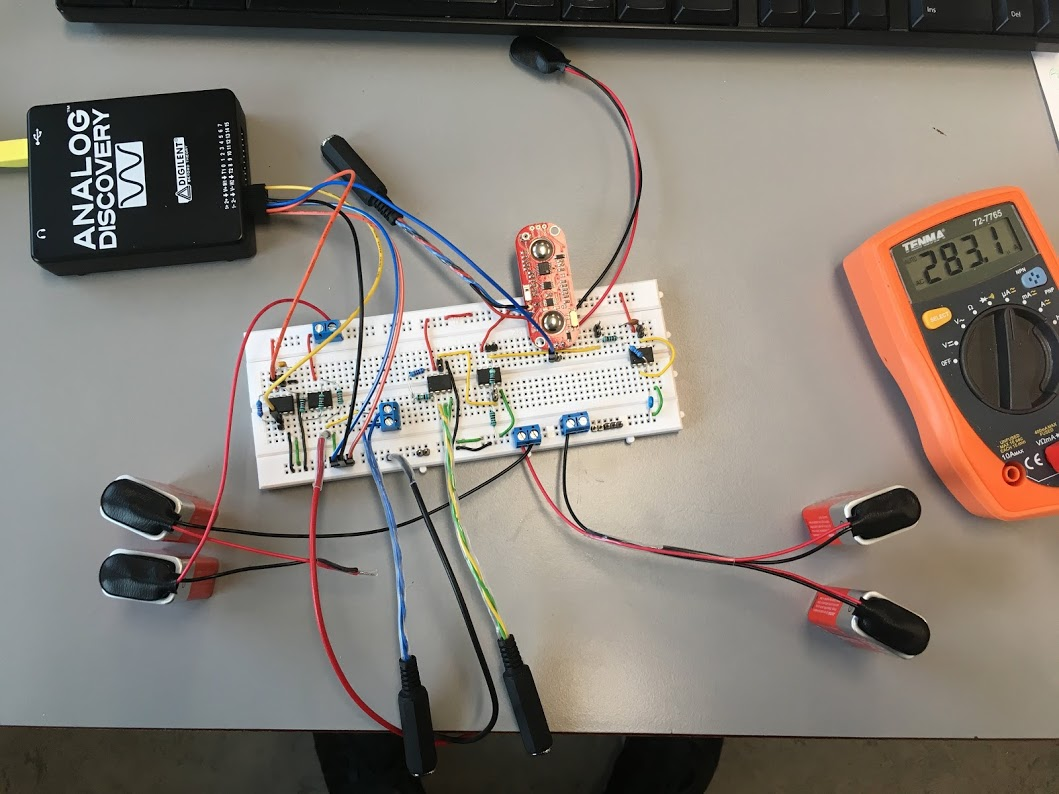
\includegraphics[width=12cm]
{Figure/integrationstestBilleder1}}
\caption{Et foto af alle komponenter implementeret på et fumlebræt. }
\label{fig:integrationstestBilleder1}
\end{figure} 


Figur \ref{aaspectrumimplementering} viser delsystemer, som er bygget på fumlebrættet. Her er der forsøgt at gøre ledninger så pæne så muligt. 

\begin{figure}[H] 
\centering
{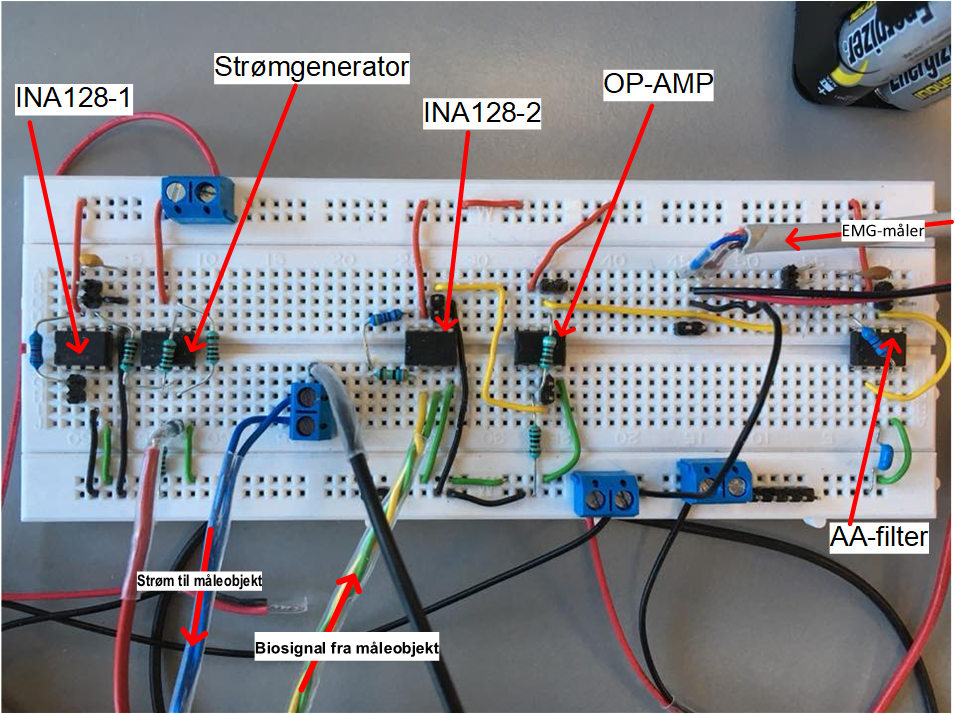
\includegraphics[width=10cm]
{Figure/aaspectrumimplementering}}
\caption{Et nært billede af, hvordan SRM'en er bygget på et fumlebræt.}
\label{aaspectrumimplementering}
\end{figure}



\pagebreak

\section{Software}

På baggrund af designfasen for SRM'ens software kan implementeringen påbegyndes. Til implementering  af systemet software-del benyttes  udviklingsværktøjet/scriptsproget  Matlab pga. følgende fordele:


\begin{itemize}
\item Matlab forærer databehandlingsfunktioner som ligger klar til anvendelse
\item Matlab er god til at indlæse store mængde data med få kodelinjer
\item I Matlab kan man udvikle en brugergrænseflade nemt og hurtigt 
\item Ved brug af Matlab med Analog Discovery, kan man betjene  funktionsgeneratoren, dataopsamlingsenheden og brugergrænsefladen  fra ét sted
\end{itemize}
   
Med disse fordele var det oplagt at vælge Matlab som både udviklingsmiljø og programmeringssprog.  
Kodeimplementeringen er organiseret i små funktioner, som kan kaldes på tværs af hinanden. Implementering af koden tager højde for at koden kan udvides uden at det påvirker andre dele af systemet. Nedenunder ses en Callback knap, der indeholder en række funktioner, som er implementeret i hver sin script-fil og kaldes, når knappen aktiveres af brugeren ved at trykke på den. Én af disse funktioner er funktionen $"Process-Measurements"$, som indeholder kodestykker, der behandler data. Behandlingen af data sker i en bestemt sekvens, som kan udtrykkes vha. et aktivitets diagram, se \ref{Fig:designUML}. 

\lstinputlisting[frame=single, firstline=96, lastline=105]{matlabkode/Synkerefleksmonitor.m}


\lstinputlisting[frame=single]{matlabkode/Process_Measurements.m}

\begin{figure}[H]
\centering
{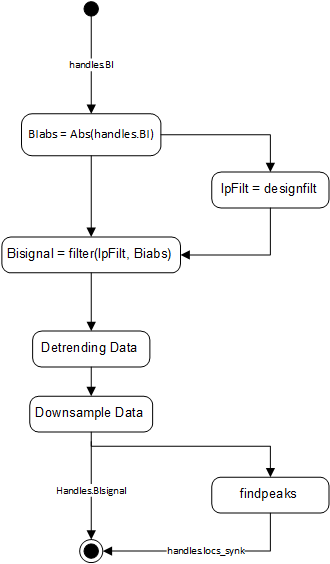
\includegraphics[width=8cm]
{Figure/designUML}}
\caption{Figuren viser indholdet af kodeeksekvering i funktionen \textit{"Process\_Measurements"} i den del hvor der udføres envelope af det rå BI-signal. Først bliver det rå BI signal dobbeltensrettet og dernæst filtreret vha. digital lavpasfilter med knækfrekvens = 500 Hz og dæmper med 40 dB over en dekade. Til sidst bliver signalet detrended, downsampled og synk detekteres.}
\label{Fig:designUML}
\end{figure} 

Yderligere beskrivelse af de resterende Callbacks og funktioner, henvises der til \nameref{bilag6}. 
